% Options for packages loaded elsewhere
\PassOptionsToPackage{unicode}{hyperref}
\PassOptionsToPackage{hyphens}{url}
%
\documentclass[
]{article}
\usepackage{amsmath,amssymb}
\usepackage{iftex}
\ifPDFTeX
  \usepackage[T1]{fontenc}
  \usepackage[utf8]{inputenc}
  \usepackage{textcomp} % provide euro and other symbols
\else % if luatex or xetex
  \usepackage{unicode-math} % this also loads fontspec
  \defaultfontfeatures{Scale=MatchLowercase}
  \defaultfontfeatures[\rmfamily]{Ligatures=TeX,Scale=1}
\fi
\usepackage{lmodern}
\ifPDFTeX\else
  % xetex/luatex font selection
\fi
% Use upquote if available, for straight quotes in verbatim environments
\IfFileExists{upquote.sty}{\usepackage{upquote}}{}
\IfFileExists{microtype.sty}{% use microtype if available
  \usepackage[]{microtype}
  \UseMicrotypeSet[protrusion]{basicmath} % disable protrusion for tt fonts
}{}
\makeatletter
\@ifundefined{KOMAClassName}{% if non-KOMA class
  \IfFileExists{parskip.sty}{%
    \usepackage{parskip}
  }{% else
    \setlength{\parindent}{0pt}
    \setlength{\parskip}{6pt plus 2pt minus 1pt}}
}{% if KOMA class
  \KOMAoptions{parskip=half}}
\makeatother
\usepackage{xcolor}
\usepackage[margin=1in]{geometry}
\usepackage{graphicx}
\makeatletter
\def\maxwidth{\ifdim\Gin@nat@width>\linewidth\linewidth\else\Gin@nat@width\fi}
\def\maxheight{\ifdim\Gin@nat@height>\textheight\textheight\else\Gin@nat@height\fi}
\makeatother
% Scale images if necessary, so that they will not overflow the page
% margins by default, and it is still possible to overwrite the defaults
% using explicit options in \includegraphics[width, height, ...]{}
\setkeys{Gin}{width=\maxwidth,height=\maxheight,keepaspectratio}
% Set default figure placement to htbp
\makeatletter
\def\fps@figure{htbp}
\makeatother
\setlength{\emergencystretch}{3em} % prevent overfull lines
\providecommand{\tightlist}{%
  \setlength{\itemsep}{0pt}\setlength{\parskip}{0pt}}
\setcounter{secnumdepth}{-\maxdimen} % remove section numbering
\newlength{\cslhangindent}
\setlength{\cslhangindent}{1.5em}
\newlength{\csllabelwidth}
\setlength{\csllabelwidth}{3em}
\newlength{\cslentryspacingunit} % times entry-spacing
\setlength{\cslentryspacingunit}{\parskip}
\newenvironment{CSLReferences}[2] % #1 hanging-ident, #2 entry spacing
 {% don't indent paragraphs
  \setlength{\parindent}{0pt}
  % turn on hanging indent if param 1 is 1
  \ifodd #1
  \let\oldpar\par
  \def\par{\hangindent=\cslhangindent\oldpar}
  \fi
  % set entry spacing
  \setlength{\parskip}{#2\cslentryspacingunit}
 }%
 {}
\usepackage{calc}
\newcommand{\CSLBlock}[1]{#1\hfill\break}
\newcommand{\CSLLeftMargin}[1]{\parbox[t]{\csllabelwidth}{#1}}
\newcommand{\CSLRightInline}[1]{\parbox[t]{\linewidth - \csllabelwidth}{#1}\break}
\newcommand{\CSLIndent}[1]{\hspace{\cslhangindent}#1}
\usepackage{setspace}
\setstretch{1.5}
\ifLuaTeX
  \usepackage{selnolig}  % disable illegal ligatures
\fi
\IfFileExists{bookmark.sty}{\usepackage{bookmark}}{\usepackage{hyperref}}
\IfFileExists{xurl.sty}{\usepackage{xurl}}{} % add URL line breaks if available
\urlstyle{same}
\hypersetup{
  pdftitle={Pre-Analysis Plan: Gender Bias in Wikipedia Articles of Politicians},
  pdfauthor={Hannah Schweren},
  hidelinks,
  pdfcreator={LaTeX via pandoc}}

\title{Pre-Analysis Plan: Gender Bias in Wikipedia Articles of
Politicians}
\author{Hannah Schweren}
\date{2024-01-22}

\begin{document}
\maketitle

{
\setcounter{tocdepth}{2}
\tableofcontents
}
\hypertarget{summary}{%
\section{1. Summary}\label{summary}}

The project aims to measure gender bias in politicians' Wikipedia
biographies. Wikipedia ranks as the seventh most visited website
worldwide in 2022
(\href{https://www.statista.com/statistics/1201880/most-visited-websites-worldwide/}{Statista
2023}), with over 4 billion unique global visitors per month
(\href{https://www.statista.com/statistics/1259907/wikipedia-website-traffic/}{Statista
2023}). Many individuals rely on it to quickly access information about
celebrities, artists, and politicians. Therefore, it is crucial for
Wikipedia's content to maintain neutrality and avoid reinforcing
societal biases. One could argue that this importance is heightened
within the subgroup of politicians, as Wikipedia's representation of
political figures influences citizens seeking information before
elections in democratic processes. Previous research has revealed a
noticeable lexical gender bias in Wikipedia biographies. I specifically
focus on politicians' biographies to investigate whether general
findings can be applied to this specific subgroup. Additionally, much of
the existing research concentrates on English articles, whereas I
analyze all politicians' texts in their respective national languages.
This approach potentially allows to compare the extent of gender bias
across different countries. My research questions are as follows:

\textbf{RQ1:} Can results of previous research concerning lexical gender
bias in biographies be applied to the subgroup of (german) politican's
biographies?

Depending on capacity, a second question will be examined, focusing on
the international perspective:

\textbf{RQ2:} Do the outcomes across different countries accurately
mirror the gender inequalities present in those countries' real-world
situations?

I plan to address these questions using available data from the
``Comparative Legislator Database,'' (Göbel and Munzert 2022) which
includes information about politicians, their Wikipedia names, and
additional details such as traffic and edits from nine countries (`aut,'
`can,' `cze,' `esp,' `fra,' `deu,' `irl,' `sco,' `gbr,' `usa\_house,' or
`usa\_senate'). Initially, I will retrieve all articles in their
original language and then assess the extent of gender bias in the
articles, first using simple descriptive indicators and secondly either
employing mutual pointwise information or a machine learning approach.
The results will be contextualized using existing research.

\hypertarget{motivation-and-background}{%
\section{2. Motivation and background}\label{motivation-and-background}}

\textbf{``Representation of the world, like the world itself, is the
work of men; they describe it from their own point of view, which they
confuse with absolute truth.''} -- Simone de Beauvoir

This research topic is particularly intriguing to me, as I have been
interested in gender equality topics for several years now. During my
studies, I have delved into the concept of the child penalty and worked
on addressing the gender care gap in my student job. These experiences
have motivated me to explore gender-related inequalities further. In the
scope of my master's thesis at Hertie School, I aim to look deeper into
such issues in the online world and utilize the techniques I have
acquired during my studies. Thus, this research topic is very exciting
for me, and I am curious to dive deeper into gender inequalities in the
political area. As a public policy student, the category of politicians
is specifically interesting to me. Inequalities in this sphere are
particularly noteworthy as politicians online representation impacts
people's perception of them and thus has a real-life impact in
democratic processes. So, misrepresentation in the form of gender bias
can be seen as problematic for democratic processes, as citizens use
online platforms like Wikipedia to inform themselves, expecting a
neutral voice. I expect to acquire skills in the field of text data
processing, which will be advantageous for my future career. I aspire to
work in the political sphere after my graduation, and a lot of political
data is in the form of text. Thus, I hope to gain some knowledge that
will be useful for my next steps after university.

\hypertarget{introduction}{%
\section{3. Introduction}\label{introduction}}

Gender bias can be defined as ``the term used to describe systematic
biasing effects that result from gender-related stereotyping and
prejudice.'' (Leibniz Association 2023) The rise of gender studies and
research about those systematic effects revealed the existence of
various such biases against women. There is studies on gender bias in
academia (European Research universities 2018) at the workplace (Heilman
2012), in medicine (Mendelsohn 1994), sports (Eastman and Billings
2000), in politics (Chiao, Bowman, and Gill 2008) - and this list could
go on. Research has for example shown variations in the adjectives used
to describe women compared to those used for men across various contexts
(Trix and Psenka 2003). While sometimes those biases are rather easy to
detect, the field of Wikipedia,as an encyclopedia is particularly
interesting, as it feigns objectivity. Wikipedia is an online source,
produced and revised by volunteers globally. Thus, it is not far fetched
to expect societal biases reflected in its articles, often this might be
unconscious, as individuals often engage in discriminatory behaviors
without conscious intent, acting upon internalized schemas (European
Research universities 2018). Furter, research has shown that an
overwhelming majority of editors are male: Less than 13\% of Wikipedia
contributors are female. (Antin et al. 2011)

``Throughout human history, a disproportionate degree of political power
around the world has been held by men.'' (Chiao, Bowman, and Gill 2008,
1) Thus, it is important to find sources and ways to reduce gender bias,
starting by detecting its existence. There is a growing body of research
on gender bias in politics, as the proportion of male to female
politicians is often very uneven (Kumar 2014). Even though this presence
of gender gaps in private and public leadership positions has long been
identified and efforts have been taken to change this, the following
statement from (Chiao, Bowman, and Gill 2008) still holds to this day.

The area of research focusing on gender bias in wikipedia has developed
in the last few years and is mainly focussed on English articles and
general biographies (not focusing on one specific category of people).
The following 3 papers are of a main interest, when dealing with lexical
gender bias on wikipedia:

\textbf{1. ``Women through the glass ceiling: gender asymmetries in
Wikipedia''} (Wagner et al. 2016) aim at assessing potential gender
inequalities in English Wikipedia articles along different dimensions
using the The DBpedia dataset. Adopting an open vocabulary approach,
they consider n-grams with \(n \leq 2\) 2 to encompass multi-word
concepts. The analysis involves exploring the association between the
top 200 n-grams for each gender and the four topics (gender,
relationship, family, or other), with Pointwise Mutual Information used
for ranking the n-grams for men and women. Among other findings, they
achieve to show that family-, gender-, and relationship-related topics
are more present in biographies about women, which is a clear indicator
for a lexical bias.

\textbf{2. ``First Women, Second Sex: Gender Bias in Wikipedia''}
(Graells-Garrido, Lalmas, and Menczer 2015) deal with the question
wether there is a gender bias in in Wikipedia and if so, how to identify
and quantify it. For this, they use the DBPedia 2014 dataset and The
Wikipedia English Dump of October 2014. They rely on several approaches
to estimate the gender bias in the articles, among others they use
Pointwise mutual information and find that ``Sex-related content is more
frequent in women biographies than men's, while cognition-related
content is more highlighted in men biographies than women's''.

\textbf{3. ``It's a Man's Wikipedia? Assessing Gender Inequality in an
Online Encyclopedia'' (Wagner et al. 2021)} As in the previous paper,
Wagner et al.~assess potential gender inequalities in Wikipedia articles
along different dimensions (coverage bias, structural bias, lexical bias
and visibility bias). In this paper they also include several language
editions and compare their results with the Gender Inequality Index of
the World Economic Form (WMF) (Forum, n.d.) to draw a connection between
bias in the offline and online world. The authors use collections of
notable people as reference datasets, crawling the articles for the
dataset's individuals. To assess the amount of lexical bias, they,
again, use an open vocabulary approach. Instead of an analysis of the
PMI, as in the previous paper, they use tfidf scores to train a Naive
Bayes classifier. Further, they employ log likelihood ratios (L(word,
g)) to assess which words are most effective in discerning the gender of
the person mentioned in an article.The lexical analysis shows ``that
articles about women tend to emphasize the fact that they are about a
women (\ldots) while articles about men don't contain words like
``man'', ``masculine'' or ``gentleman''.'' (Wagner et al. (2021), p.458)

\hypertarget{research-question}{%
\section{4. Research question}\label{research-question}}

The main research question is the following:

\textbf{RQ1: Can results of previous research concerning lexical gender
bias in biographies be applied to the subgroup of (german) politican's
biographies?}

I will begin the analysis with german text and if there is enough
capacity, also include other countries Potentially, the international
perspective will be elaborated with a second research question:

\textbf{RQ2: Do the outcomes across different countries accurately
mirror the gender inequalities present in those countries' real-world
situations?}

The approach reflects previous research on this topic, specifying the
examined group, focusing on politicians, instead of generic biographies
on wikipedia. I will mainly examine lexical gender bias, meaning,
different language representation of females and males which is one of
many possible kinds of biases (Coverage Bias, visibility bias etc.)

\textbf{Hypotheses}

H1: The findings from previous research about all categories of
biographies can be applied to politicians. As demonstrated in the
Finkbeiner test (Finkbeiner 2013), women's biographies are expected to
emphasize their gender, whereas descriptions of men are presented as
neutral.

\hypertarget{data-and-methods}{%
\section{5. Data and methods}\label{data-and-methods}}

\textbf{Data:}

I am using the data of the Comparative legislature Database (Göbel and
Munzert (2022)), containing information (including sex, wikititle,
traffic, edits etc.) on more than 67,000 contemporary and historical
legislators. To gather the according wikipedia articles of the
politicians, I use the wikipediR package. I use a subset of politicians
that don't have a date of death recorded in the data and thus are
contemporarian politicians, as I am rather interested in the gender bias
towards politicians that are known as (acting) politicians, not as
historical figures. The data includes 10 available countries: Canada,
Germany, France, Czech Republic, USA, Ireland, Scotland, Austria and
Spain. Figure 1 gives an overiew of structure of the database

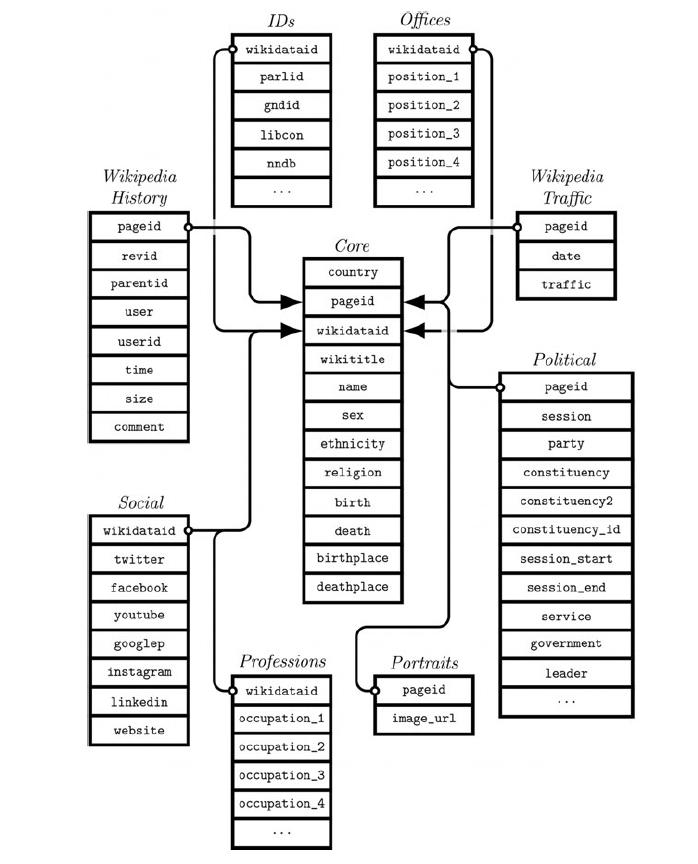
\includegraphics{Overview_cld.png}.

Figure 1: Structure of the database (Göbel and Munzert 2022, 7)

\textbf{Method:}

\textbf{Decriptive analyis}

The start of the analysis will be a descriptive analysis of the
available data. Figures like the length of the articles have already
been used in previous research to get an impression of possible bias
(Graells-Garrido, Lalmas, and Menczer (2015)). For my analysis, I plan
to use the average monthly page traffic as a matching variable to only
include comparable female and male politicians. This serves the purpose
of reducing the influence of possible confounders - I expect the biggest
confounder in this case to be the popularity of certain politicians.
Monthly page traffic seems like a good proxy to reduce this confounding
factor. Further, I want to compare not only the article length but also
the number of page edits of the female and male politicians.

\textbf{Further analysis}

The descriptive analysis will be followed by a technique to detect
gender bias in the text, focusing on the kind of bias that is pretty
common based on previous research (Wagner et al. (2016)), namely lexical
bias. Lexical bias means that language is used differently when talking
about men/women (Lakoff 1973). I want to propose two possible methods to
analyse the extend of lexical bias in politicians biographies. Depending
on the complexity of the method, a focus on one or few countries may be
advantageous (e.g.~focusing on German politicians and or compare to
one/few other countries) as the methods have to be applied to each
country individually.

\textbf{Option 1}

The method to detect gender bias is inspired by (Wagner et al. 2016) and
has been used by other authors as well to assess lexical bias
(Graells-Garrido, Lalmas, and Menczer 2015) For this method, Pointwise
Mutual Information (PMI) is used to find out which words are strongly
associated with articles of females/males.

Previous research has often focused on the Wikipedia introduction text
to detect bias. In my analysis, I plan to include the whole text as I
expect the introduction texts for politicians to be rather simple,
similar and short, whereas the other sections include more relevant
information for the analysis.

\begin{itemize}
\tightlist
\item
  First step of this approach is to tokenize the wikipedia articles and
  to create the vocabulary, containing ``gender'', ``word'' and ``Number
  of biographies'' containing this word.
\item
  Next, stopwords are removed, and only words that are present in both
  genders are included.
\item
  After creating a dataframe that contains all common words of female
  and male politicians, with the respective frequency for men/women, the
  PMI scores for the vocabulary are calculated. PMI is expressed as:
  \(\text{PMI}(c, w) = \log \frac{p(c, w)}{p(c)p(w)}\) C represents the
  gender and w represents the word.
\item
  Further, the PMI score needs to be normalized for further analysis.
\item
  PMI gives extra weight to words with very low frequencies thus I need
  to establish a threshold for words to be included. PMI helps identify
  words that tend to occur together with a specific gender term more
  frequently than expected by chance - so, higher PMI values indicate a
  stronger association between a word and a specific gender.
\item
  The next step is thus to sort the resulting PMI values decreasingly
  for each gender.
\item
  Following the approach tested by (Wagner et al. 2016), the top 200
  words are manually annotated and put in categories: Family,
  Relationship, Gender, Other.
\item
  To assess differences between the genders, a chi-square test is used
  for the categories of men and women. Further, word Clouds or other
  visualization techniques can be used to show the results of the
  analysis for each gender.
\end{itemize}

\textbf{Alternative}

The second possible method is a machine learning approach as applied by
(Wagner et al. 2021)or (Brun et al. 2022) before.

\begin{itemize}
\tightlist
\item
  Again, this is an open vocabulary approach.
\item
  Firstly, it includes stemming the words of the wikipedia articles and
  creatign a corpus with wikipedia articles categorized by gender
\item
  Then, Term Frequency-Inverse Document Frequency scores (tfidf Scores)
  are computed, used to evaluate the importance of a word in a document
  relative to a collection of documents (corpus).
\item
  These Scores are used as features to train a Naive Bayes classifier,
  which serves the purpose of identifying words that effectively
  differentiate the gender of the individual discussed in an article.
\item
  After identifying these important discriminative features by assessing
  feature importance, the same method as above can be used to annotate
  and categorize the words.
\end{itemize}

\textbf{International analysis}

As I am particularly interested in the German case, as a German speaker
and having gained experiences in gender inequalities in Germany, I will
firstly apply the respective methods to the German language. If there is
enough capacity to apply the method to several countries, I will
continue with English and French speaking countries (as I speak those
languages and I am able to annotade words myself). An alternative would
be to group all countries with the same language (e.g.~Germany and
Austria) but as I ideally aim to compare my results on a country level,
I decided against this option. If I can apply my method to several
countries, I aim at comparing the country level of gender equality,
measured by the Gender Inequality Index of the World Economic Form (WMF)
(forum 2023) with the results of my lexical bias analyis to see, if
there is a connection. This way of comparing bias in the offline world
and the bias on Wikipedia has been conducted by (Wagner et al. 2021)
before.

\hypertarget{bibliographie}{%
\section{Bibliographie:}\label{bibliographie}}

\hypertarget{refs}{}
\begin{CSLReferences}{1}{0}
\leavevmode\vadjust pre{\hypertarget{ref-antin_gender_2011}{}}%
Antin, Judd, Raymond Yee, Coye Cheshire, and Oded Nov. 2011. {``Gender
Differences in {Wikipedia} Editing.''} In \emph{Proceedings of the 7th
{International} {Symposium} on {Wikis} and {Open} {Collaboration}},
11--14. Mountain View California: ACM.
\url{https://doi.org/10.1145/2038558.2038561}.

\leavevmode\vadjust pre{\hypertarget{ref-brun_wikigender_2022}{}}%
Brun, Natalie Bolón, Sofia Kypraiou, Natalia Gullón Altés, and Irene
Petlacalco Barrios. 2022. {``Wikigender: {A} {Machine} {Learning}
{Model} to {Detect} {Gender} {Bias} in {Wikipedia}.''} arXiv.
\url{http://arxiv.org/abs/2211.07520}.

\leavevmode\vadjust pre{\hypertarget{ref-chiao_political_2008}{}}%
Chiao, Joan Y., Nicholas E. Bowman, and Harleen Gill. 2008. {``The
{Political} {Gender} {Gap}: {Gender} {Bias} in {Facial} {Inferences}
That {Predict} {Voting} {Behavior}.''} Edited by Laurie Santos.
\emph{PLoS ONE} 3 (10): e3666.
\url{https://doi.org/10.1371/journal.pone.0003666}.

\leavevmode\vadjust pre{\hypertarget{ref-eastman_sportscasting_2000}{}}%
Eastman, Susan Tyler, and Andrew C. Billings. 2000. {``Sportscasting and
{Sports} {Reporting}: {The} {Power} of {Gender} {Bias}.''} \emph{Journal
of Sport and Social Issues} 24 (2): 192--213.
\url{https://doi.org/10.1177/0193723500242006}.

\leavevmode\vadjust pre{\hypertarget{ref-leagur_of_european_research_universities_implicit_2018}{}}%
European Research universities, Leagur of. 2018. {``Implicit Bias in
Academia: {A} Challenge to the Meritocratic Principle and to Women's
Careers -- {And} What to Do about It,''} Advice {Paper}, January.
\url{https://www.leru.org/files/Publications/Implicit-bias-in-academia-Full-Paper.pdf}.

\leavevmode\vadjust pre{\hypertarget{ref-finkbeiner_what_2013}{}}%
Finkbeiner, Ann. 2013. {``What {I}'m {Not} {Going} to {Do}.''} \emph{The
Last Word On Nothing}.
\url{https://www.lastwordonnothing.com/2013/01/17/5266/}.

\leavevmode\vadjust pre{\hypertarget{ref-world_economic_forum_global_2023}{}}%
forum, World Economic. 2023. {``Global {Gender} {Gap} {Report} 2023.''}

\leavevmode\vadjust pre{\hypertarget{ref-world_economic_forum_global_nodate}{}}%
Forum, World Economic. n.d. {``Global {Gender} {Gap} {Report} 2023.''}

\leavevmode\vadjust pre{\hypertarget{ref-gobel_comparative_2022}{}}%
Göbel, Sascha, and Simon Munzert. 2022. {``The {Comparative}
{Legislators} {Database}.''} \emph{British Journal of Political Science}
52 (3): 1398--408. \url{https://doi.org/10.1017/S0007123420000897}.

\leavevmode\vadjust pre{\hypertarget{ref-graells-garrido_first_2015}{}}%
Graells-Garrido, Eduardo, Mounia Lalmas, and Filippo Menczer. 2015.
{``First {Women}, {Second} {Sex}: {Gender} {Bias} in {Wikipedia}.''} In
\emph{Proceedings of the 26th {ACM} {Conference} on {Hypertext} \&
{Social} {Media} - {HT} '15}, 165--74.
\url{https://doi.org/10.1145/2700171.2791036}.

\leavevmode\vadjust pre{\hypertarget{ref-heilman_gender_2012}{}}%
Heilman, Madeline E. 2012. {``Gender Stereotypes and Workplace Bias.''}
\emph{Research in Organizational Behavior} 32 (January): 113--35.
\url{https://doi.org/10.1016/j.riob.2012.11.003}.

\leavevmode\vadjust pre{\hypertarget{ref-kumar_participation_2014}{}}%
Kumar, Dr Pankaj. 2014. {``Participation of {Women} in {Politics}:
{Worldwide} Experience.''}

\leavevmode\vadjust pre{\hypertarget{ref-lakoff_language_1973}{}}%
Lakoff, Robin. 1973. {``Language and {Woman}'s {Place}.''}
\emph{Language in Society} 2 (1): 45--80.
\url{http://www.jstor.org/stable/4166707}.

\leavevmode\vadjust pre{\hypertarget{ref-leibniz_association_gender_2023}{}}%
Leibniz Association. 2023. {``Gender {Bias} {In} {Academia} {And}
{Research}.''} \emph{Center of Excellence Women and Science}.
\url{https://www.gesis.org/en/cews/data-and-information/research-areas/gender-bias}.

\leavevmode\vadjust pre{\hypertarget{ref-mendelsohn_sex_1994}{}}%
Mendelsohn, Kathleen D. 1994. {``Sex and {Gender} {Bias} in {Anatomy}
and {Physical} {Diagnosis} {Text} {Illustrations}.''} \emph{JAMA: The
Journal of the American Medical Association} 272 (16): 1267.
\url{https://doi.org/10.1001/jama.1994.03520160051042}.

\leavevmode\vadjust pre{\hypertarget{ref-trix_exploring_2003}{}}%
Trix, Frances, and Carolyn Psenka. 2003. {``Exploring the {Color} of
{Glass}: {Letters} of {Recommendation} for {Female} and {Male} {Medical}
{Faculty}.''} \emph{Discourse \& Society} 14 (2): 191--220.
\url{https://doi.org/10.1177/0957926503014002277}.

\leavevmode\vadjust pre{\hypertarget{ref-wagner_its_2021}{}}%
Wagner, Claudia, David Garcia, Mohsen Jadidi, and Markus Strohmaier.
2021. {``It's a {Man}'s {Wikipedia}? {Assessing} {Gender} {Inequality}
in an {Online} {Encyclopedia}.''} \emph{Proceedings of the International
AAAI Conference on Web and Social Media} 9 (1): 454--63.
\url{https://doi.org/10.1609/icwsm.v9i1.14628}.

\leavevmode\vadjust pre{\hypertarget{ref-wagner_women_2016}{}}%
Wagner, Claudia, Eduardo Graells-Garrido, David Garcia, and Filippo
Menczer. 2016. {``Women Through the Glass Ceiling: Gender Asymmetries in
{Wikipedia}.''} \emph{EPJ Data Science} 5 (1): 5.
\url{https://doi.org/10.1140/epjds/s13688-016-0066-4}.

\end{CSLReferences}

\end{document}
